\documentclass{article}

% TODO code als voorbeeld op het web

\newcommand{\longversion}[1]{}
\newcommand{\shortversion}[1]{#1}

\usepackage{graphicx}
\usepackage{listings}
\usepackage{url}

%% for normal spacing
\usepackage{spconf}

%% for double spacing
%\usepackage[left=2cm,top=3cm,right=2cm]{geometry} 
%\usepackage{setspace}
%\doublespacing


%\title{How to Build a Correlator with Many-Core Hardware}
\title{Building Correlators with Many-Cores}

%% for normal spacing
\name{Rob V. van Nieuwpoort and John W. Romein}
\address{Stichting ASTRON (Netherlands Institute for Radio Astronomy) \\
Oude Hoogeveensedijk 4, 7991 PD\ \ Dwingeloo, The Netherlands \\
\texttt{\{nieuwpoort,romein\}@astron.nl}
}

%% for double spacing
%\author{Rob V. van Nieuwpoort and John W. Romein \\ 
%Stichting ASTRON (Netherlands Institute for Radio Astronomy) \\
%Oude Hoogeveensedijk 4, 7991 PD\ \ Dwingeloo, The Netherlands \\
%\texttt{\{nieuwpoort,romein\}@astron.nl}
%}



\begin{document}

\maketitle

\begin{abstract}
Radio telescopes typically consist of multiple receivers whose
signals are cross-correlated to filter out noise.  A recent trend
is to correlate in software instead of custom-built hardware, taking
advantage of the flexibility that software solutions offer.  Examples
include e-VLBI and LOFAR.  However, the data rates are usually high
and the processing requirements challenging.  Many-core processors are
promising devices to provide the required processing power.

In this paper, we explain how to implement and optimize
signal-processing applications on multi-core CPUs and many-core
architectures, such as the Intel Core i7, NVIDIA and ATI GPUs, and the
\mbox{Cell/B.E.}  We use correlation as a running example. The
correlator is a streaming, possibly real-time application, and is much
more I/O intensive than applications that are typically implemented on
many-core hardware today.  We compare with the LOFAR production
correlator on an IBM Blue Gene/P supercomputer.  We discuss several
important architectural problems which cause architectures to perform
suboptimally, and also deal with programmability.

The correlator on the Blue Gene/P achieves a superb 96\% of the
theoretical peak performance.  We show that the processing power and
memory bandwidth of current GPUs are highly imbalanced. Because of
this, the correlator achieves only 16\% of the peak on ATI GPUs, and
32\% on NVIDIA GPUs.  The \mbox{Cell/B.E.} processor, in contrast,
achieves an excellent 92\%.  Many of the insights we discuss here are not only
applicable to telescope correlators, are valuable when developing
signal-processing applications in general.
\end{abstract}


\section{Introduction}
% wat gaat de lezer leren van dit paper?

% we geven een leidraad voor het kiezen van de juiste architectuur voor het probleem van de lezer
% voor goede performance heb je nodig:
%  - kennis van algorithme
%  - kennis van de architecturen
%  - inzicht over hoe je de mapping van algorithme op architectuur het beste kunt doen
% dit paper geeft inzicht in de verschillen tussen architecturen, en inzicht over welke factoren belangrijk zijn om de mapping goed te doen.

Radio telescopes produce enormous amounts of data.
The \emph{Low-Frequency Array\/} (LOFAR)~\cite{deVos:09}, for instance, will produce some tens
of petabits per day, and the \emph{Australian SKA Pathfinder\/} will
even produce over six exabits per day~\cite{askap}.
These modern radio telescopes use many separate receivers as building blocks,
and combine their signals to form a single large and sensitive instrument.

To extract the sky signal from the system noise, the \emph{correlator\/}
correlates the signals from different receivers, and integrates the
correlations over time, to reduce the amount of data.
This is a challenging problem in radio astronomy,
since the data volumes are large, and the computational demands grow
quadratically with the number of receivers.
Correlators are not limited to astronomy, but are also used 
in geophysics~\cite{correlator-geophysics},
radar systems~\cite{correlator-radar}, 
wireless networking~\cite{correlator-wireless}, etc.

Traditionally, custom-built hardware, and later FPGAs were used to correlate telescope signals.
A recent development is to use a supercomputer~\cite{ppopp2010}.
Both approaches have important advantages and disadvantages.
Custom-built hardware is efficient and consumes modest amounts of power, but is
inflexible, expensive to design, and has a long development time.
Solutions that use a supercomputer are much more flexible, but are less
efficient, and consume more power. %, and are expensive to purchase and maintain.
Future instruments, like the Square Kilometre Array (SKA), need several orders
of magnitude more computational resources.
It is likely that the requirements of the SKA cannot be met by using
current supercomputer technology. Therefore, it is important to investigate
alternative hardware solutions.

General-purpose architectures no longer
achieve performance improvements by increasing the clock frequency, but
by adding more compute cores and by exploiting parallelism.  Intel's
recent Core~i7 processor is a good example of this. It has four
cores and supports additional vector parallelism.
Furthermore, the high-performance computing community is
steadily adopting clusters of Graphics Processor Units (GPUs) as a viable
alternative to supercomputers, due to their unparalleled growth in
computational performance, increasing flexibility and programmability,
high power efficiency, and low purchase costs.
GPUs are highly parallel and contain hundreds of processor cores.
%% However, their usefulness is often limited to applications that do not require
%% double-precision floating-point arithmetics, since there is no need for
%% double-precision calculations to play games.
%% Hence, the support for double-precision arithmetic is typically poor.
%% Fortunately, many signal-processing applications do not require double
%% precision.
An example of a processor that combines GPU and CPU
qualities into one design is the Cell Broadband Engine~\cite{cell}.
The \mbox{Cell/B.E.} consists of an ``ordinary'' PowerPC core and eight powerful
vector processors that provide the bulk of the processing power.
Programming the \mbox{Cell/B.E.} requires more effort than programming an ordinary CPU,
but various studies showed that the \mbox{Cell/B.E.} performs well on
signal-processing tasks like FFTs~\cite{fftc}.

In this article, we explain how many-core architectures can be
exploited for signal-processing purposes.  We give
insights into their architectural limitations, and how to best cope
with them.  We treat five different, popular architectures with
multiple cores: the \mbox{Cell/B.E.}, GPUs from both NVIDIA and ATI, the Intel Core i7 processor, and
the IBM Blue Gene/P (BG/P) supercomputer.  We discuss their
similarities and differences, and how the architectural differences
affect optimization choices and the eventual performance of a
correlator. We also discuss the programmability of the architectures.
We focus on correlators, but many of the
findings, claims, and optimizations hold for other signal-processing
algorithms as well, both inside and outside the area of radio astronomy.
For instance, we discuss another signal-processing algorithm, radio-astronomy imaging, on many-core
hardware elsewhere~\cite{gridding}. 
%, but this
%paper should be of special interest to those who are willing to invest
%some extra programming effort to obtain good performance, even if
%high-level programming support is not available.
In this paper, we use the LOFAR telescope as a running example, and
use its production correlator on the BG/P as a comparison. This way,
we demonstrate how many-core architectures can be used in practice for a real
application.
For educational purposes, we made the correlator implementations for all architectures available online.
They exemplify the different optimization choices for the different architectures.
The code may be reused under the GNU public license.
%\emph{Note to the reviewers: we will do so soon, but the code needs additional documentation to be instructive.}
We describe and analyze the correlator on many-core
platforms in much more detail in~\cite{Nieuwpoort:09}. 


\section{Trends in radio astronomy}

During the past decade, new types of radio-telescope concepts emerged that
rely less on concrete, steel, and extreme cooling techniques, but more on
signal-processing techniques.
For example, LOFAR~\cite{deVos:09}, MeerKAT (Karoo Array Telescope)~\cite{meerkat} and
ASKAP (Australian Square Kilometre Array Pathfinder)~\cite{askap}
are distributed sensor networks
that combines the signals of many receiver elements.
All three are pathfinders for the future SKA (Square Kilometre Array)~\cite{ska} telescope, which
will be orders of magnitude larger.
%Also, aperture array tiles like Embrace~\cite{embrace} and focal plane arrays
%like Apertif~\cite{apertif} are novel multi-receiver concepts.
%Unlike single-pixel feeds from traditional dish-based telescopes, 
These
instruments combine the advantages of higher sensitivity, higher resolution,
and multiple concurrent observation directions.
But, they require huge
amounts of processing power to combine the data from the receiving elements.

The signal-processing hardware technology used to process telescope
data also changes rapidly.  Only a decade ago, correlators required
special-purpose ASICs to keep up with the high data rates and
processing requirements.  The advent of sufficiently fast FPGAs
significantly lowered the developments times and costs of
correlators, and increased the flexibility
substantially. LOFAR requires even more flexibility to support many
different processing pipelines for various observation modes, and uses
FPGAs for on-the-field processing and a BG/P
supercomputer to perform real-time, central processing.
We describe LOFAR in more detail below.

%  dit past hier niet
%% Recent many-core architectures seem to be a viable complement to the aforementioned processing platforms.
%% GPUs provide more processing power and are more power-efficient than CPUs,
%% while GPUs are more flexible and easier to program than FPGAs.
%% Since GPUs of different vendors are mutually quite different, we did an
%% extensive performance comparison between the architectures of popular GPUs 
%% for signal-processing purposes, particularly, for correlation
%% purposes~\cite{Nieuwpoort:09}.


\subsection{The LOFAR telescope}

\begin{figure}[t]
\vspace{-0.4cm}
\begin{center}
\includegraphics[width=60mm]{figures/LBA-field.jpg}
\end{center}
\vspace{-0.5cm}
\caption{A field with LOFAR antennas.}
\label{fig:lba-field}
\end{figure}

\begin{figure*}[t]
\begin{minipage}[b]{11cm}
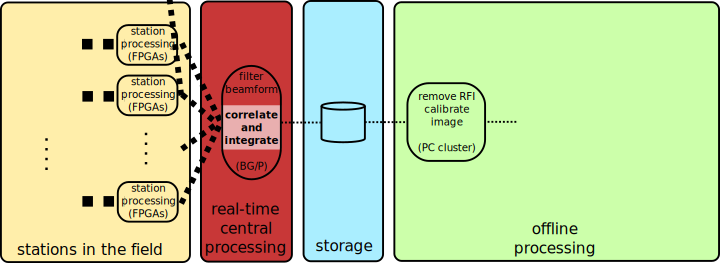
\includegraphics[width=11cm]{figures/lofar-overview.pdf}
\caption{A simplified overview of the LOFAR processing.}
\label{fig:lofar-overview}
\end{minipage}
\hfill
\begin{minipage}[b]{55mm}
\includegraphics[width=\columnwidth]{figures/map.jpg}
\caption{Possible LOFAR layout.}
\label{fig:map}
\end{minipage}
\end{figure*}

LOFAR is an aperture array radio telescope operating in the
10 to 250~MHz frequency range~\cite{deVos:09}.  It is the first of a new generation of
radio telescopes, that breaks with the concepts of traditional
telescopes in several ways.  Rather than using large, expensive
dishes, LOFAR uses many thousands of simple antennas that have no
movable parts, see
Figure~\ref{fig:lba-field}.  Essentially, it is a distributed sensor
network that monitors the sky and combines all signals centrally.
This concept requires much more signal processing, but the 
costs of the silicon for the processing are much lower that the costs of steel that would
be needed for dishes. Moreover, LOFAR can observe the sky in many
directions concurrently and switch directions instantaneously.  In
several ways, LOFAR will be the largest telescope of the world.
The antennas are simple, but there are a lot of them: 44000 in the full LOFAR
design. To make radio pictures of the sky with adequate resolution,
these antennas are to be arranged in clusters.
In the rest of this paper, we call a cluster of antenna's \emph{a receiver}.
The receivers will be spread out over
an area of ultimately 350 km in diameter. This is shown in Figure~\ref{fig:map}.
%In the current phase, 31.000 antenna's with a maximum distance of 100 km will
%be built. 
Data transport requirements are in the range of many
tera-bits/sec and the processing power needed is tens of tera-ops.

Another novelty is the elaborate
use of \emph{software\/} to process the telescope data in real time.
%The signals from the
%antennas are digitised, transported to a central location,
%and combined in software to emulate a conventional instrument. 
LOFAR thus is an IT-telescope. 
The cost
is dominated by the cost of computing and will follow Moore's law,
becoming cheaper with time and allowing increasingly large telescopes
to be built. 
\longversion{
LOFAR will enable exciting new science cases.  First, we expect to see
the \emph{Epoch of Reionization\/} (EoR), the time that the first star
galaxies and quasars were formed. Second, LOFAR offers a unique
possibility in particle astrophysics for studying the origin of
high-energy \emph{cosmic rays}.  Third, LOFAR's ability to
continuously monitor a large fraction of the sky makes it uniquely
suited to find new \emph{pulsars} and to study \emph{transient
  sources}.  Since LOFAR has no moving parts, it can instantaneously
switch focus to some galactic event.  Fourth, \emph{Deep Extragalactic
  Surveys\/} will be carried out to find the most distant radio
galaxies and study star-forming galaxies.  Fifth, LOFAR will be
capable of observing the so far unexplored radio waves emitted by
\emph{cosmic magnetic fields}.  For a more extensive description of
the astronomical aspects of the LOFAR system, see De Bruyn
et.~al.~\cite{Bruyn:02}.
}
A global overview of the LOFAR processing is given in
Figure~\ref{fig:lofar-overview}. The thickness of the lines indicates
the size of the data streams.  Initial processing is done in the
field, using FPGA technology.  Typical operations that are performed
there include analog-to-digital conversion, filtering, frequency
selection, and combination of the signals from the different
antenna's.  Next, the data is transported to the central processing
location in Groningen via dedicated optical wide-area networks.

The real-time central processing of LOFAR data is done on
a BG/P supercomputer.  There, we filter the data, and
perform phase shift and bandpass corrections.
Next, the signals from all stations are cross-correlated.  The
correlation process performs a data reduction by integrating samples
over time.  Finally, the data is forwarded to a storage cluster, where
results can be kept for several days.  After an observation has
finished, further processing, such as RFI removal, calibration, and imaging is done off-line, on commodity cluster
hardware.  
In this paper, we focus on the correlator step (the
highlighted part in the red box in
Figure~\ref{fig:lofar-overview}), because it must deal with the
full data streams from all receivers. Moreover, its costs grow
quadratically with the number of receivers, while all other steps have
a lower time complexity.


\section{Correlating signals}
\label{sec:correlating}


%XF vs FX. lofar is FX. Met een groter aantal inputs is FX efficienter?
%transpose


%% \begin{figure*}[t]
%% \begin{center}
%% 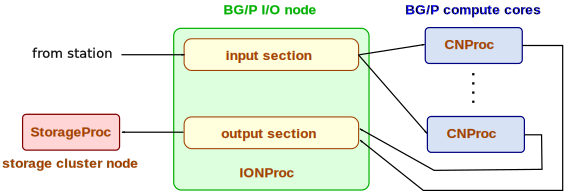
\includegraphics[width=12cm]{figures/processing-overview.pdf}
%% \end{center}
%% \vspace{-0.5cm}
%% \caption{A simplified view of LOFAR processing.}
%% \label{fig-processing-overview}
%% \end{figure*}


%The data streams from the receivers contain samples, which are complex
%numbers that represent the amplitude and phase of a signal.  
LOFAR's receivers are dual-polarized; they take separate
samples from orthogonal (X and Y) directions.  The receivers
support 4, 8 and 16 bit integer samples, where the normal mode of
operation uses the 16 bit samples to help mitigate the impact of strong RFI. The smaller samples are important
for observations that require larger sky coverage. 
Before filtering and correlating, the
samples are converted to single-precision floating point, since all
architectures support this well.  This is
accurate enough for our purposes. From the perspective of the
correlator, samples thus consist of \emph{four} 32-bit floating point
numbers: two polarizations, each with a real and an imaginary part.

LOFAR uses an FX correlator: it first filters the different frequencies, and
then correlates the signals. This is more efficient than an XF correlator for larger numbers of receivers.
\longversion{
Prior to correlation, the data that comes from
the receivers must be reordered:
each input carries the signals of many frequency bands from a single
receiver, but the correlator needs data from a single frequency of all inputs.
Depending on the data rate, switching the data can be a real challenge.
The data reordering phase is outside the scope of this paper, but a correlator
implementation cannot ignore this issue.
The LOFAR Blue Gene/P correlator uses the fast 3D~torus for this purpose;
other multi-core architectures need external switches.
}
The received signals from sky sources are so weak, that the antennas 
mainly receive noise. To see if there is statistical coherence
in the noise, simultaneous samples of each pair of receivers are correlated, 
by multiplying the sample of one receiver with the complex
conjugate of the sample of the other receiver.
To reduce the output size, the correlations are integrated over time, by accumulating all products. 
Therefore, the correlator is mostly multiplying and adding complex numbers.
Both polarizations of a station A are correlated with both polarizations 
of a station B, yielding correlations in XX, XY, YX, and YY
directions.
The correlator algorithm itself thus is straightforward, and can be
written in a single formula: \\
$C_{s_1,s_2\geq s_1,p_1\in\{X,Y\},p_2\in\{X,Y\}} = \displaystyle\sum_{t} Z_{s_1,t,p_1} * Z_{s_2,t,p_2}^\ast$ 

The total number of correlations we have to compute is $(nrReceivers \times
(nrReceivers + 1)) / 2$, since we need each pair of correlations only
once. This includes the autocorrelations (the correlation of a receiver with itself),
since we need them later in the pipeline for calibration purposes.
The autocorrelations can be computed with less instructions.
We can implement the correlation operation very efficiently, with only
four fused-multiply-add (fma) instructions, doing eight floating-point
operations in total. For each pair of receivers, we have to do this
four times, once for each combination of polarizations. Thus, in total
we need 32 operations. To perform these operations, we have to load
the samples generated by two different receivers from memory.  As
explained above, the samples each consist of four single-precision
floating-point numbers.  Therefore, we need to load 8 floats or 32 bytes in
total.  This results in \emph{exactly one FLOP/byte}. 
We will describe the implementation and optimization of the correlator on the
many-core systems in more detail in Section~\ref{sec:optimizing}, but first, we explain the architectures themselves. 


\section{Many-core architectures}

\begin{table*}[t]
\begin{center}
%{\footnotesize % for normal layout
{\scriptsize % for double spaced
\begin{tabular}{|l|l|l|l|l|l|}                                                   
\hline
Architecture                                 & Intel Core i7 & IBM Blue Gene/P& ATI 4870 &  NVIDIA Tesla C1060 & STI Cell/B.E. \\
\hline
\textbf{gflops per chip}                     & \textbf{85}   & \textbf{13.6}  & \textbf{1200}  & \textbf{936}  & \textbf{204.8}\\
Clock frequency (GHz)                        & 2.67          & 0.850          & 0.75           & 1.296         & 3.2           \\
cores x FPUs per core = \textbf{total FPUs}  & 4 x 4 = \textbf{16} & 4 x 2 = \textbf{8} & 160 x 5 = \textbf{800} & 30 x 8 = \textbf{240} & 8 x 4 = \textbf{32} \\
%operations per cycle per FPU                & 2             &   2            & 2              & 2             & 2             \\
%\hline
registers per core x register width          & 16 x 4        & 64 x 2         & 1024 x 4      & 2048 x 1       & 128 x 4       \\
%\hline
%total L1 data cache size per chip (KB)      & 32            & 128            & undisclosed   & undisclosed    & 2048          \\
%total L1 cache bandwidth (GB/s)             & undisclosed   & 54.4           & 480           & undisclosed    & 409.6         \\
total device RAM bandwidth (GB/s)            & n.a.          & n.a.           & 115.2         & 102            & n.a.          \\
\textbf{total host RAM bandwidth (GB/s)}     & \textbf{25.6} & \textbf{13.6}  & \textbf{4.6}  & \textbf{5.6}   & \textbf{25.8} \\
%\hline
%Process Technology (nm)                      & 45            & 90             & 55            & 65             & 65            \\
%TDP (W)                                      & 130           & 24             & 160           & 236            & 70            \\
%\textbf{gflops / Watt (based on TDP)}       & \textbf{0.65} & \textbf{0.57}  & \textbf{7.50} & \textbf{3.97}  & \textbf{2.93} \\
%\hline
%\textbf{gflops/device bandwidth (gflops / GB/s)}& n.a.       &  n.a.          & \textbf{10.4} & \textbf{9.2}   & n.a.         \\
%\textbf{gflops/host bandwidth (gflops / GB/s)} & \textbf{3.3}& \textbf{1.0}   & \textbf{150}  & \textbf{117}   & \textbf{7.9} \\
\hline
\end{tabular}
} %\small
\end{center}
\vspace{-0.5cm}
\caption{Properties of the different many-core platforms.}
\label{architecture-properties}
\end{table*}

%% \begin{table*}
%% \begin{center}
%% \begin{small}
%% \begin{tabular}{|l|rrrrrr|}
%% \hline
%% & GTX~280 & RV770 & Cell BE & BG/P & Core i7 920 & Larrabee \\
%% \hline
%% peak performance (GFLOPS) & 936 & 1,200 & 205(SPEs) + 25.6(PPU) & 13.6 & 85 & ? \\
%% clock (GHz) & 1,3 & 0.75 & 3.2 & 0.85 & 2.67 & ? \\
%% \#cores & 240 & 800 & 8 & 4 & 4 & $\mathcal{O}$(10) \\
%% \#threads/core & & & 1 & 1 & 2 & 4 \\
%% L1 cache size/core (KiB) & & & 256 (I+D) & 32(I) + 32(D) & 32(I) + 32(D) & \\
%% L2 cache size/core (KiB) & & & & 2 (prefetcher) & 256 (I+D) & \\
%% L3 cache size/chip (MiB) & & & & 8 & 8 & \\
%% (device) memory size (GiB) & 4 & &  & 2 or 4 & & \\
%% peak memory bandwidth (GiB/s) & 102 & 115.2 & & & & \\
%% \#registers/core & & & 128 & 32 & 16 & 32 \\
%% \#floats/register (= vector size) & 1 & 1  & 4 & 2 & 4 & 16 \\
%% manufacturing process (nm) & 65 & & & 90 & 45 & \\
%% Thermal Design Power (Watt) & 236 & 160 & & & 130 & \\
%% \hline
%% \end{tabular}
%% \end{small}
%% \end{center}
%% \end{table*}

In this section, we explain key properties of five different
architectures with multiple cores, and the most important differences between them. 
Table~\ref{architecture-properties}
shows the most important properties of the different many-core
architectures. 


\noindent \\ \emph{General Purpose multi-core CPUs (Intel Core i7)}

\noindent As a reference, we implemented the correlator on a multi-core
general-purpose architecture, in this case an Intel Core~i7.  The
theoretical peak performance of the system is 85~gflops, in single
precision.  The parallelism comes from four cores with 
hyperthreading.
Using two threads per core allows the hardware to overlap
load delays and pipeline stalls with useful work from the other thread.
The SSE4 instruction set provides SIMD (Single Instruction, Multiple Data) parallelism with a vector length of four floats.

%% SSE4 does not provide fused multiply-add instructions, but the Core~i7
%% issues vector-multiply and vector-add instructions concurrently in
%% different pipelines, allowing eight flops per cycle per core.  

\noindent \\ \emph{IBM Blue Gene/P supercomputer}

\noindent The IBM Blue Gene/P~\cite{IBM:08} is the architecture that is
currently used for the LOFAR correlator.
Four PowerPC processor cores are integrated on each BG/P chip.
Each core is extended with two floating-point units, that provide the bulk of the processing power.
The BG/P is an energy-efficient supercomputer.
This is accomplished by using many small, low-power chips, at a low clock
frequency.
%The supercomputer also has excellent I/O capabilities, there are five
%specialized networks for communication.


\noindent \\ \emph{ATI GPUs}

\noindent ATI's GPU with the highest performance is
the Radeon 4870~\cite{amd-manual}.  The chip contains 160 cores, with 800 FPUs in total, 
and has a theoretical peak performance of
1.2~teraflops. The board uses a PCI-express~2.0 interface
for communication with the host system.
The GPU has 1 GB of device memory on-board.
It is possible to specify if a read should be
cached by the texture cache or not.
Each streaming processor also has 16 KB of shared
memory that is completely managed by the application. 
On both ATI and NVIDIA GPUs, the application should run many more threads
than the number of cores. This allows the hardware to overlap memory load delays with useful
work from other threads.


\noindent \\ \emph{NVIDIA GPUs}

\noindent NVIDIA's Tesla C1060 contains a GTX~280 GPU with 240 single
precision and 30 double precision FPUs~\cite{cuda-manual}. The GTX~280
uses a two-level hierarchy to group cores.  There are 30~independent
\emph{multiprocessors\/} that each have 8~cores.  Current NVIDIA GPUs
have fewer cores than ATI GPUs, but the individual cores are faster.
The theoretical peak performance is 933 gflops.  The number of
registers is large: each multiprocessor has 16384 32-bit floating point registers,
that are shared between all threads that run on it.
There also is 16~KB of shared memory per
multiprocessor.  Finally, texture-caching hardware
is available.  The application can specify which area of device memory
must be cached, while the shared memory is completely managed by the
application.



\noindent \\ \emph{The Cell Broadband Engine}

\noindent The \mbox{Cell/B.E.}~\cite{cell} is a
heterogeneous many-core processor, designed by Sony, Toshiba and IBM
(STI).  The \mbox{Cell/B.E.} has nine cores: one Power Processing
Element (PPE), acting as a main processor, and eight Synergistic
Processing Elements (SPEs) that provide the real processing power.
%The cores, the main memory, and the external I/O are connected by a
%high-bandwidth element interconnection bus.
%The PPE's main role is to
%run an operating system and to coordinate the SPEs.  
An SPE contains
a RISC core, a 256KB Local Store (LS), and a DMA controller.
The LS is an extremely fast local memory for both code and data
and is managed \emph{entirely by the application} with explicit DMA
transfers to and from main memory.  The LS can be considered the SPU's (explicit) L1 cache.  The
\mbox{Cell/B.E.} has a large number of registers: each SPU has 128,
which are 128-bit (4 floats) wide.
\longversion{
 The SPU can dispatch two
instructions in each clock cycle using the two pipelines designated
\emph{even} and \emph{odd}. Most of the arithmetic instructions
execute on the even pipe, while most of the memory instructions
execute on the odd pipe. 
}
For the performance evaluation, we use a QS21 Cell blade with two
\mbox{Cell/B.E.} processors.
The 8 SPEs of a single chip in the
system have a total theoretical single-precision peak performance of
205 gflops.


\section{Mapping signal-processing algorithms on many-core hardware}

Many-core architectures derive their performance from parallelism.
Several different forms of parallelism can be identified:
multi-threading (with or without shared memory), overlapping of I/O
and computations, instruction-level parallelism, and vector parallelism. Most
many-core architectures combine several of these methods.  
Unfortunately, an application has to handle all available levels of parallelism to
obtain good performance.
Therefore, it is clear that algorithms have to be adapted to efficiently exploit
many-core hardware.
Additional parallelism can be obtained by using multiple processor chips.
In this paper, however, we restrict ourselves to single chips for simplicity.



\subsection{Finding parallelism}

The first step is to find parallelism in the algorithm, on all
different levels.  Basically, this means looking for independent
operations.  With the correlator, for example, the thousands of
different frequency channels are completely independent, and can be
processed in parallel. But there are other, more fine-grained sources
of parallelism as well.  The correlations for each pair of stations
are independent, just like the four combinations of  
polarizations.  Finally, samples taken at different times can
be correlated independently, as long as the sub-results are integrated
later. Of course, the problem now is how to map the parallelism in the
algorithm to the parallelism provided by the architecture. We found
that, even for the relatively straightforward correlator algorithm,
the different architectures require very different mappings and
strategies.


\subsection{Optimizing memory pressure and access patterns}

On many-core architectures, the memory bandwidth is shared between the
cores.  This has shifted the balance between between computational and
memory performance.  The available memory bandwidth \emph{per operation} has
decreased dramatically compared to traditional processors.  For the
many-core architectures we use here, the theoretical bandwidth per operation is
3--10 times lower than on the BG/P, for instance. In practice, if algorithms
are not optimized well for many-core platforms, the achieved memory bandwidth can
easily be ten to a hundred times lower than the theoretical maximum.
Therefore, we must
treat memory bandwidth as a scarce resource, and it is important to
minimize the number of memory accesses.  In fact, one of the most
important lessons of this paper is that on many-core architectures,
optimizing the memory properties of the algorithms is more important
than focusing on reducing the number of compute cycles that is used,
as is traditionally done on systems with only a few or just one core.

\begin{table}[t]
\begin{center}
{\footnotesize
\begin{tabular}{|l|l|l|}
\hline
feature                   & Cell/B.E.                      & GPUs \\
\hline
access times              & uniform                        & non-uniform \\
\hline
cache sharing level       & single thread (SPE)            & all threads in a \\
                          &                                & multiprocessor \\
\hline
access to off-chip mem.   & through DMA only               & supported \\
\hline
mem. access overlapping   & asynchronous DMA               & hardware-managed \\
                          &                                & thread preemption \\
\hline
communication             & DMA between SPEs               & independent thread  \\
                          &                                & blocks \& shared   \\
                          &                                & mem. within a block \\
\hline
\end{tabular}
} %\small
\end{center}
\vspace{-0.5cm}
\caption{Differences between memory architectures.}
\label{memory-properties}
\end{table}



\subsubsection{Well-known memory optimization techniques}

The insight that optimizing the interaction with the memory system is
becoming more and more important is not new.  The book by Catthoor et
al.~\cite{data-access} is an excellent starting point for more
information on memory-system related optimizations. 
%The authors focus
%on multimedia applications, but the techniques described there are
%also applicable to the field of signal processing, which has many
%similarities to multimedia.

We can make a distinction between hardware and software memory
optimization techniques.  Examples of hardware-based techniques include caching, data
prefetching, write combining, and pipelining. The software techniques can be divided
further into compiler optimizations and algorithmic improvements.
  The distinction between hardware and
software is not entirely black and white. Data prefetching, for
instance, can be done both in harware and software.  Another good
example is the explicit cache of the \mbox{Cell/B.E.} processor. This is
an architecture where the programmer handles the cache
replacement policies instead of the hardware.

Many optimizations focus on utilizing data caches more efficiently.
Hardware cache hierarchies can, in principle, transparently improve application performance.
Nevertheless, it is important to take the sizes of the
different cache levels into account when optimizing an algorithm.  A
cache line is the smallest unit of memory than can be transferred
between the main memory and the cache.  Code can be optimized for the
cache line size of a particular architecture.  Moreover, the
associativity of the cache can be important.  If a cache is N-way set
associative, this means that any particular location in memory can be
cached in either of N locations in the data cache. Algorithms can be
designed such that they take care that cache lines that are needed
later are not replaced prematurely. 
In addition, write combining,
a technique that allows data writes to be combined and written later in burst mode,
can be used if the ordering of writes is not important.
Finally, prefetching can be used to load data into caches or registers ahead of time.

Many cache-related optimization techniques have been described in the
literature, both in the context of hardware and software. For
instance, an efficient implementation of hardware-based prefetching is
described in~\cite{Chen95effectivehardware-based}.  As we will
describe in Section~\ref{sec:optimizing}, we implemented prefetching
manually in software, for example by using multi-buffering on the
\mbox{Cell/B.E.}, or by explicitly loading data into shared memory or
registers on the GPUs.  A good starting point for cache-aware or
cache-oblivious algorithms is~\cite{cache}. An example of a technique
that we used to improve cache efficiencies for the correlator is the
padding of multi-dimensional arrays with extra ``dummy'' data
elements.  This can be especially important if memory is accessed with
a stride of a (large) power of two.  This way, we can make sure that
cache replacement policies work well, and subsequent elements in an
array dimension are not mapped onto the same cache location.  This
well-known technique is described, for instance, by Bacon et
al.~\cite{cache-tlb-compiler}.  Many additional data access patterns
optimization techniques are described in~\cite{data-access}.

Many memory optimization techniques have been developed in the context
of optimizing compilers and runtime systems (e.g., efficient memory allocators). 
For instance, a lot of research effort has been invested in cache-aware memory allocation; see
e.g.,~\cite{Wilson95dynamicstorage}.  Compilers can exploit many
techniques to optimize locality, by applying code and loop
transformations such as interchange, reversal, skewing, and
tiling~\cite{data-locality}.  Furthermore, compilers can optimize code for
the parameters and sizes of the caches, by carefully choosing the
placement of variables, objects, and arrays in
memory~\cite{Panda96memorydata}.

The memory systems of the many-core architectures are quite
complex. GPUs, for instance, have banked device memory, several levels of texture cache,
in addition to local memory, application-managed
shared memory (also divided over several banks), and write combining buffers.
There also are complex interactions between the memory
system and the hardware thread scheduler.
GPUs literally run tens of thousands of parallel threads
to overlap memory latencies, trying to keep all functional units fully occupied.
We apply the techniques described
above in software by hand, since we found that the current compilers
for the many-core architectures do not (yet) implement them well on
their complex memory systems.


% OpenCL helpt misschien, door runtime compilation.

\subsubsection{Appying the techniques}

So, the second step of mapping a signal-processing algorithm to a many-core architecture
is optimizing the memory behavior. We can split this step into two phases:
an algorithm phase and an architectural phase.
In the first phase, we identify algorithm-specific, but
architecture-independent optimizations. 
In this phase, it is of key importance to understand that, although a
set of \emph{operations} in an algorithm can be independent, the \emph{data
  accesses} may not be.  This is essential for good performance, even though it may not be a
factor in the correctness of the algorithm. The \emph{number} of memory accesses per operation should
be reduced as much as possible, sometimes even at the cost of more
compute cycles. An example is a case
where different parallel operations read (but not write) the
same data.  For the correlator, the most important insight here
is a technique to exploit date reuse opportunities, reducing the number of memory
loads. We explain this in detail in Section~\ref{sec:tiling}.

The second phase deals with architecture-specific optimizations.
In this phase, we do not reduce the \emph{number} of memory loads, but think about the
memory \emph{access patterns}. Typically, several cores share one or
more cache levels. Therefore, the access patterns of several different
threads that share a cache should be tailored accordingly. On GPUs,
for example, this can be done by \emph{coalescing} memory accesses.
This means that different concurrent threads read subsequent memory
locations.  This can be counter-intuitive, since traditionally, it was
more efficient to have linear memory access patterns within a
thread. Table~\ref{memory-properties} summarizes the differences in
memory architectures of the different platforms.
Other techniques that are performed in this phase include optimizing cache
behavior, avoiding load delays and pipeline stalls, exploiting special floating-point instructions, etc.
We explain several examples of this in more detail in Section~\ref{sec:architecture-optimizations}.


\subsection{A simple analytical tool}

A simple analytic approach, the Bound and Bottleneck
analysis~\cite{system-performance,roofline}, can provide more insight
on the memory properties of an algorithm. It also gives us a reality
check, and calculates what the expected maximal performance is that can be
achieved on a particular platform.
The number of operations that is performed per byte that have to be
transferred (the flop/byte ratio) is called the \emph{arithmetic intensity}, or
$AI$~\cite{system-performance}.  Performance is bound by the product
of the bandwidth and the $AI$: 
$\mathit{perf_{max}}$ = $AI \times bandwidth$. 
Several important assumptions are made
with this method. First, it assumes that the bandwidth is
independent of the access pattern.  Second, it assumes a complete
overlap of communication and computation, i.e., all latencies
are completely hidden.  Finally, the method does not take caches into
account. Nevertheless, it gives a rough idea of
the performance than can be achieved.

It is insightful to apply this method to the correlator on the GPUs.
We do it for the NVIDIA GPU here, but the results for the ATI hardware is similar.
With the GPUs, there are several communication steps that influence
the performance. First, the data has to be transferred from the host to
the device memory.  Next, the data is read from the device memory into
registers. The host-to-device bandwidth is limited by the low
PCI-express throughput, 5.6 GB/s in this case. We can easily show that this is a bottleneck
by computing the $AI$ for the full system, using the host-to-device transfers. (The AI can also be computed for
the device memory.)
 
As explained in Section~\ref{sec:correlating}, the number of flops in the correlator is the
number of receiver combinations times 32 operations, while the number
of bytes that have to be loaded in total is 16 bytes times the number
of receivers.  The
number of combinations is $(nrReceivers \times (nrReceivers + 1)) / 2$ (see Section~\ref{sec:correlating}).
If we substitute this, we find that the $AI = nrReceivers + 1$.  For
LOFAR, we can assume 64 receivers (each in turn containing many
antennas), so the $AI$ is 65 in our case.  Therefore, the performance
bound on NVIDIA hardware is $65 \times 5.6 = 363$ gflops. This is only
39\% of the theoretical peak.  Note that this even is optimistic,
since it assumes perfect overlap of communication and computation.
%The efficiency can improve if additional processing is performed on the GPU 
%(e.g., a filter step before the correlator) and intermediate data is kept in device memory.

\subsection{Complex numbers}

\longversion{
Programming languages like C99 and FORTRAN have native support for complex
numbers, which is useful for signal-processing applications.
Arrays of complex numbers can easily be declared like
\texttt{complex float array[16];}.
This declaration enforces real and imaginary values at alternating memory
locations.
Unfortunately, not all architectures have efficient support for complex
multiply and division operations on vector elements that are declared this
way, since these operations require real and imaginary values to be shuffled.
Moreover, the real and imaginary parts of a product are computed differently.

The Blue Gene/P is the only architecture that efficiently supports all complex
operations, while the SSE4 instructions of the Core i7 provide limited support.
To obtain good performance on the other architectures, it may be necessary
to split the complex array into separate arrays for real and imaginary values.
This increases the programming effort, since all complex operations must be
programmed in terms of real operations.
Both formats are commonly used; a library like FFTW3 supports both of them.
}

Support for complex numbers is important for signal processing. 
Explicit hardware support for complex operations is
preferable, both for programmability and performance. 
%If it is not available, we can circumvent this by using separate arrays for
%real values and for imaginary values.  
Except for the BG/P, none of the architectures support this.
The different architectures require two different approaches of
dealing with this problem. If an architecture does not use
explicit vector parallelism, the complex operations can simply
be expressed in terms of normal floating point operations. This puts
an extra burden on the programmer, but achieves good performance. The
NVIDIA GPUs work this way.  If an architecture does use vector
parallelism, we can either store the real and complex parts alternatingly inside a
single vector, or have separate vectors for the two parts.  In both
cases, support for shuffling data inside the vector registers is
essential, since complex multiplications operate on both the real and imaginary parts.
The architectures differ considerably in this
respect.  The \mbox{Cell/B.E.} excels; its vectors contain four floats, which
can be shuffled around in arbitrary patterns. Moreover, 
shuffling and computations can be overlapped effectively.  On ATI
GPUs, this works similarly.  The SSE4 instructions in the
Intel CPUs do not support arbitrary shuffling patterns.
This has a large impact on the way the code is vectorized.
%, and requires a different SIMDization strategy. 




\section{Implementation and optimization}
\label{sec:optimizing}

In this section,
we explain the techniques described above by applying them to the
correlator for all different architectures.


\subsection{Architecture independent optimizations}
\label{sec:tiling}

\begin{figure}[t]
\begin{center}
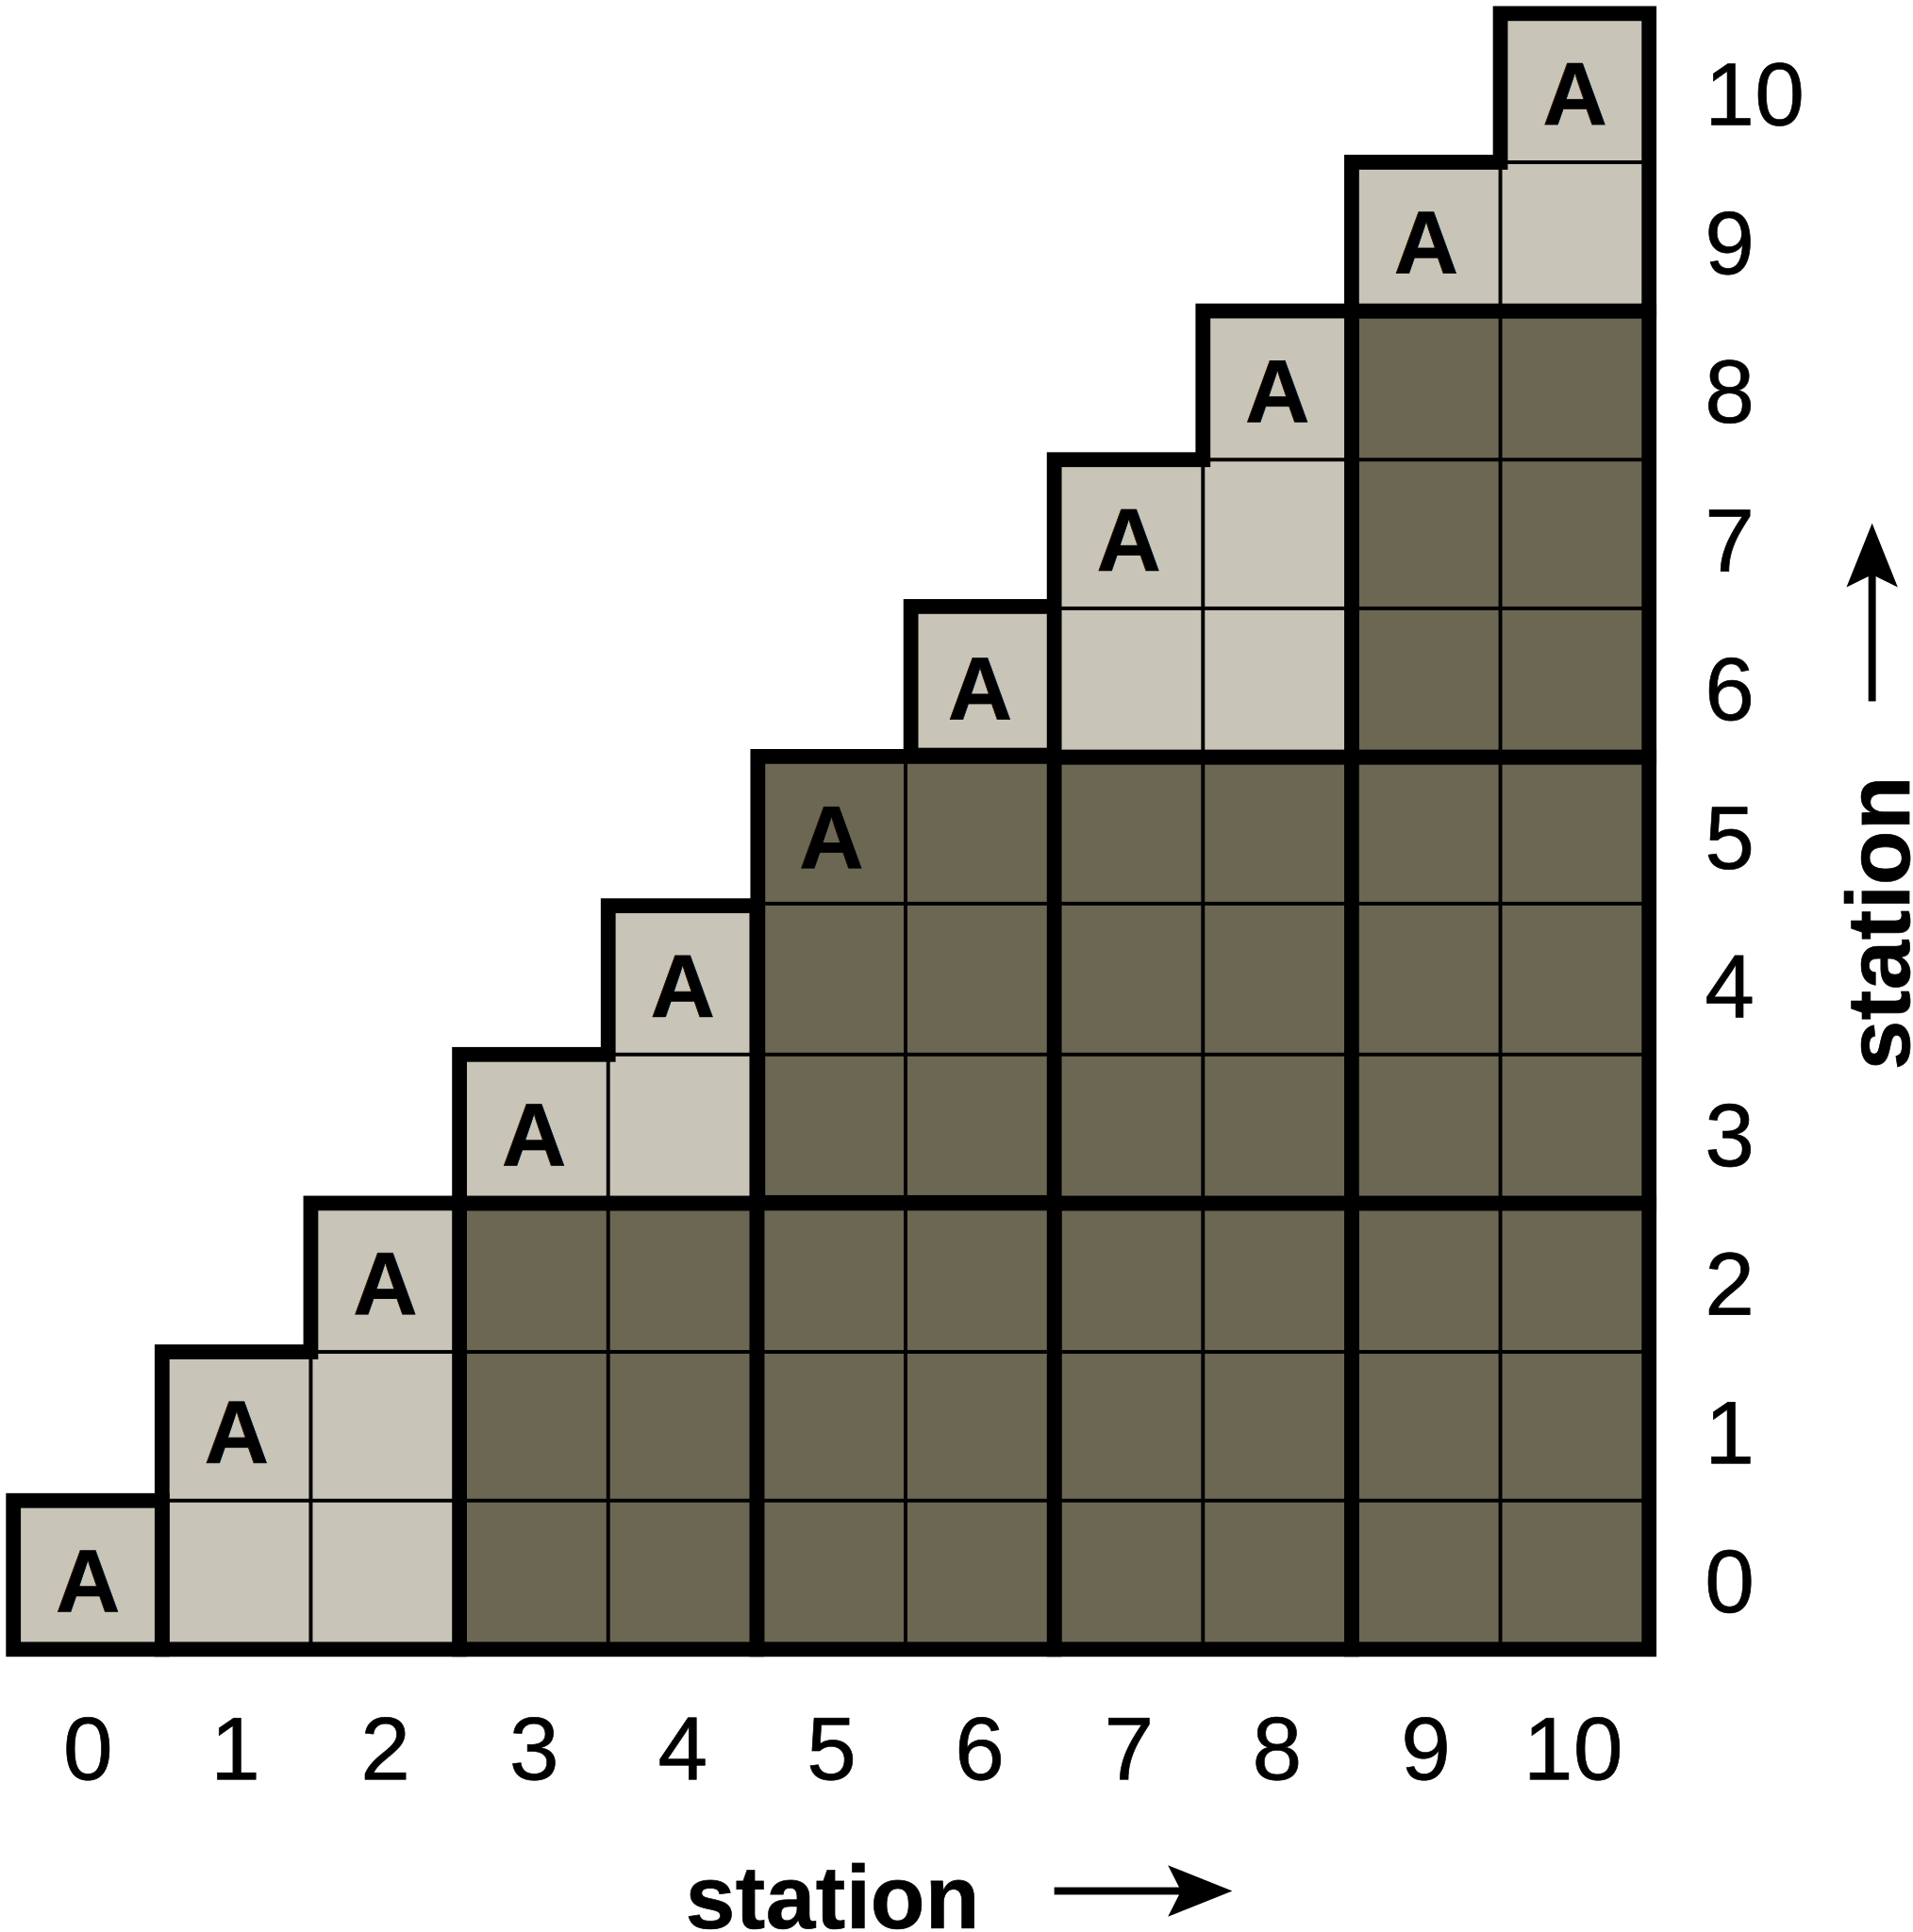
\includegraphics[width=4.2cm]{figures/correlation-triangle.pdf}
\end{center}
\vspace{-0.5cm}
\caption{An example correlation triangle.}
\label{fig-correlation}
\end{figure}

%Although in reality the receivers are dual-polarized, and the samples are complex numbers, 
%we use single-polarized real samples in the following example for simplicity.
An unoptimized correlator would read the samples from two receivers and
multiply them, requiring two sample loads for one multiplication.
We can optimize this by reusing a sample 
as often as possible, by using it for multiple correlations (see
Figure~\ref{fig-correlation}).
The figure is triangular, because we compute
the correlation of each pair of receivers only once. The squares labeled \emph{A} are
autocorrelations.
For example, the samples from receivers 8, 9, 10, and 11 can be correlated
with the samples from receivers 4, 5, 6, and 7 (the red square in the figure),
reusing each fetched sample four times.
By dividing the correlation triangle in $4\times4$ \emph{tiles}, eight samples are read from memory for sixteen
correlations, reducing the amount of memory operations by a factor
of four.
The maximum number of receivers that can
be simultaneously correlated this way (i.e., the tile size) is limited by the number of registers that an architecture has.
The samples and accumulated correlations are best kept in registers, and the number of
required registers grows rapidly with the number of receiver inputs.
The example above already requires 16 accumulators.
To obtain good performance, it is important to tune the tile size to the
architecture.
%Caches and memory prefetch units can also improve the performance.
%However, a cache-size dependent tradeoff must be made.
%On the one hand, correlating and integrating over long periods of time
%is good for pipelined FPU operation, on the other hand, the 
There still is
opportunity for additional data reuse \emph{between} tiles.  The tiles
within a row or column in the triangle still need the same samples.
In addition to registers, caches can thus also be used to increase
data reuse. 

%The efficiency of the cache, however, depends highly on the chosen 
%integration time, and on the cache-replacement algorithm 
%(Least-Recently Used works much better here than Round Robin).

%It is important to realize that the
%correlator itself is \emph{trivially parallel}, since the tens of thousands of
%frequency channels that LOFAR uses can be processed independently.  This allows us to
%efficiently exploit many-core hardware.


\begin{figure}[t]
\begin{center}
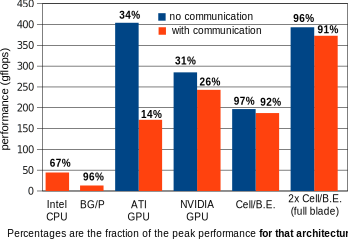
\includegraphics[width=\columnwidth]{figures/performance-graph-v2.pdf} % for normal layout
%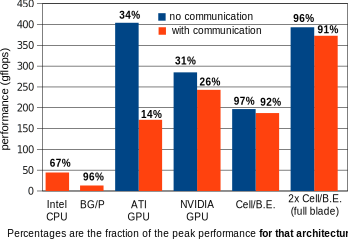
\includegraphics[width=0.5\columnwidth]{figures/performance-graph-v2.pdf} % for double spacing
\end{center}
\vspace{-0.5cm}
\caption{Achieved performance on the different platforms.}
\label{performance-graph}
\end{figure}



\subsection{Architecture-specific optimizations}
\label{sec:architecture-optimizations}

We will now describe the implementation of the correlator on
the different architectures, evaluating the performance and optimizations needed in detail. 
For comparison reasons, we use the performance
\emph{per chip} for each architecture.
%We choose 64 as the number of receivers (each in turn consisting of hundreds of antennas), since
%that is a realistic number for LOFAR.  
The performance results are shown in Figure~\ref{performance-graph}.


\noindent \\ \emph{Intel CPUs}

\noindent The SSE4 instruction set can be used to exploit vector parallelism.  
Unlike the \mbox{Cell/B.E.} and ATI GPUs, a
problem with SSE4 is the limited support for shuffling data within
vector registers.  Computing the
correlations of the four polarizations within a vector is
inefficient, and computing four samples with subsequent time stamps in a vector works
better. 
%We achieve only a speedup of a factor of 2.8 compared to
%a version without SSE4.  
%We found that, unlike on the other platforms,
%computing four samples with subsequent time stamps in a vector works
%better.  
The use of SSE4 improves the performance by a factor of 3.6
in this case.  In addition, multiple threads should be used to utilize all
four cores.  To benefit from hyperthreading, twice as many
threads as cores are needed.  For the correlator, hyperthreading increases performance by 6\%. 
Also, the number of vector registers is small.
Therefore, there is not much opportunity to reuse data in registers,
limiting the tile size to $2 \times 2$; reuse has to come from the
L1~cache.


\noindent \\ \emph{The BG/P supercomputer}

\noindent 
We found that the BG/P is extremely suitable for our application,
since it is highly optimized for processing of complex numbers.
However, the BG/P performs \emph{all} floating point operations in double
precision, which is overkill for our application.
Although the BG/P can keep the same number of values in register as the 
Intel chip, an important difference is that the BG/P has 32
registers of width 2, compared to Intel's 16 of width 4.  The smaller
vector size reduces the amount of shuffle instructions needed.
%The (small) $2 \times 2$ tile size performs best.
In contrast to all other architectures we evaluate, the problem is compute
bound instead of I/O bound, thanks to the BG/P's high memory bandwidth per
operation, which is 3--10 times higher than for the other architectures.


\noindent \\ \emph{ATI GPUs}

\noindent The ATI architecture has several important
drawbacks for data-intensive applications.  First, the
host-to-device bandwidth is a bottleneck.  Second, 
overlapping communication with computation does not work well.
We observed kernel slowdowns of more than \emph{a factor of
two} due to asynchronous transfers in the background. This can clearly be seen in Figure~\ref{performance-graph}.
Third, the architecture does not provide random write access to device
memory, but only to \emph{host} memory.
%The kernel output can be written to at most 8 output registers
%(each 4 floats wide).  For the correlator, this effectively limits the
%tile size to $2\times2$.
%Random write access to \emph{host} memory is
%provided.  
The correlator reduces the data by a large amount, and the
results are never reused by the kernel. Therefore, they can be
directly streamed to host memory. Nevertheless, in general, the absence of random
write access to device memory significantly reduces the programmability, and prohibits the use
of traditional programming models.
ATI offers two separate programming models, at different abstraction
levels~\cite{amd-manual}.  The low-level programming model is called CAL.  
It provides communication primitives and
an assembly language, allowing fine-tuning of device
performance. For high-level programming, ATI provides Brook+.  We
implemented the correlator with both models.
In both cases, the programmer has to do the vectorization,
unlike with NVIDIA GPUs.  CAL provides a feature called
\emph{swizzling}, which is used to select parts of vector registers in
arithmetic operations.  We found this improves readability of the code. 
However, the
programming tools still are unsatisfactory. The high-level Brook+ model does
not achieve acceptable performance. The low-level
CAL model does, but it is difficult to use.
The best-performing implementation uses a tile size of 4x3, thanks to
the large number of registers.  
Due to the low I/O performance, we achieve only 16\% of the theoretical peak.



\noindent \\ \emph{NVIDIA GPUs}

\noindent NVIDIA's programming model is called Cuda~\cite{cuda-manual}.
Cuda is relatively high-level, and achieves good performance.
An advantage of NVIDIA hardware, in contrast to ATI, is that the application does not have to do 
vectorization. This is thanks to the fact that all cores have their own address generation units. 
All data parallelism is expressed by using threads.
When accessing device memory, it is important to make sure that
simultaneous memory accesses by different threads are \emph{coalesced}
into a single memory transaction.  In contrast to ATI hardware, NVIDIA
GPUs support random write access to device memory. This allows a
programming model that is much closer to traditional models, greatly
simplifying software development.
It is important to use shared memory or the texture cache to enable data reuse.
In our case, we use the texture cache to speed-up access to the sample data. 
Cuda provides barrier synchronization between threads within a thread block.
We exploit this feature to let
the threads that access the same samples run in lock step.  This way,
we pay a small synchronization overhead, but we can increase the cache hit
ratio significantly.  We found that this optimization improved performance by a factor of 2.
This optimization is a good example that shows that, on GPUs, it is important to optimize
memory behavior, even at the cost of additional instructions and synchronization overhead.

\longversion{
We also investigated the use of the per-multiprocessor shared memory as an
application-managed cache.  Others report good results with this
approach~\cite{gpu-cache}.  However, we found that, for our
application, the use of shared memory only led to performance
degradation.
}

Registers are a shared resource. Using fewer registers in a kernel
allows the use of more concurrent threads, hiding load delays.
We found that using a relatively small tile size (3x2) and many threads increases performance.
The kernel itself, without host-to-device communication achieves 38\%
of the theoretical peak performance.  If we include communication, the
performance drops to 32\% of the peak. Just like with the ATI
hardware, this is caused by the low PCI-e bandwidth.  With NVIDIA
hardware significant performance gains can be achieved by using asynchronous host-to-device I/O.


\noindent \\ \emph{The Cell Broadband Engine}

\noindent With the
\mbox{Cell/B.E.} it is important to exploit all levels of parallelism.
Applications deal with task and data parallelism across multiple SPEs,
vector parallelism inside the SPEs, and multi-buffering for
asynchronous DMA transfers~\cite{cell}.  Acceptable performance can be achieved by
programming the \mbox{Cell/B.E.}  in C or C++, while using intrinsics
to manually express vector parallelism.  Thus, the programmer
specifies which instructions have to be used, but can typically leave
the instruction scheduling and register allocation to the compiler.

A distinctive property of the architecture is that cache transfers are
explicitly managed by the application, using DMA. This is unlike other 
architectures, where caches work transparently.
%% By dividing the
%% integration time into smaller intervals, we can keep the sample data
%% for \emph{all stations} in the local store.  
%% Because of this, we have to load and store the correlations to main
%% memory several times, since the sub-results have to
%% be accumulated.  
Communication can be overlapped with computation, by using multiple buffers.
Although issuing explicit DMA commands complicates programming,
we found that this usually is not problematic for signal-processing applications.
Thanks to the explicit cache,
the correlator implementation fetches each sample from main memory
\emph{only exactly once}. 
The large number of registers allows a big tile size of 
$4\times3$, leading to a lot of data reuse.
We exploit the vector parallelism of the \mbox{Cell/B.E.} by computing the four
polarization combinations in parallel.  We found that this performs
better than vectorizing over the integration time.  This is thanks to the \mbox{Cell/B.E.}'s
excellent support for shuffling data around in the vector registers.
%The shuffle instruction is executed
%in the odd pipeline, while the arithmetic is executed in the even
%pipeline, allowing them to overlap.
Due to the high
memory bandwidth and the ability to reuse data, we achieve 92\% of the peak
performance on one chip.  If we use both chips in a cell blade, we still achieve
91\%.  Even though the memory
bandwidth per operation of the \mbox{Cell/B.E.} is eight times lower than
that of the BG/P, we still achieve excellent performance, thanks to
the high data reuse factor.


\subsection{Comparison and Evaluation}
\label{sec:perf-compare}

\begin{table*}[t]
\begin{center}
%{\footnotesize % for normal layout
{\scriptsize % for double spaced
\begin{tabular}{l|l|l|l|l}
Intel Core i7 920     & IBM Blue Gene/P          & ATI 4870                      & NVIDIA Tesla C1060     & STI  Cell/B.E.                      \\
\hline
 + well-known         &  + L2 prefetch unit      &  + largest number of cores    &  + random write access &  + power efficiency                 \\
-- few registers      &  + high memory bandwidth &  + swizzling support          &  + Cuda is high-level  &  + random write access              \\
-- no fma instruction &  + fast interconnects    & -- low PCI-e bandwidth        & -- low PCI-e bandwidth &  + shuffle capabilities             \\
-- limited shuffling  & -- double precision only & -- transfer slows down kernel &                        &  + explicit cache (performance)     \\
                      & -- expensive             & -- no random write access     &                        & -- explicit cache (programmability) \\
                      &                          & -- bad programming support    &                        & -- multiple parallelism levels      \\
\end{tabular}
} %\small
\end{center}
\vspace{-0.5cm}
\caption{Strengths and weaknesses of the different platforms for signal-processing applications.}
\label{architecture-results-table}
\end{table*}

Figure~\ref{performance-graph} shows the performance on all
architectures we evaluated. The NVIDIA GPU achieves the highest
\emph{absolute} performance. Nevertheless, the GPU \emph{efficiencies}
are much lower than on the other platforms.  The \mbox{Cell/B.E.}
achieves the highest efficiency of all many-core architectures, close
to that of the BG/P. 
Although the theoretical peak performance of the
\mbox{Cell/B.E.} is 4.6 times lower than the NVIDIA chip, the absolute
performance is only 1.6 times lower.
 If both chips in the cell blade
are used, the \mbox{Cell/B.E.} also has the highest absolute
performance. For the GPUs, it is possible to use more than one chip as
well, for instance with the ATI 4870x2 device. However, we found that this does not help, since the
performance is already limited by the low PCI-e throughput, and the
chips have to share this resource.
In Table~\ref{architecture-results-table} we summarize the
architectural strengths and weaknesses that we discussed.  

%Although
%we focus on the correlator application in this paper, the
%results are applicable to signal processing applications in
%general.

%@@@ larrabee / lange vectoren

\longversion{
\section{Programmability of the platforms}

The performance gap between assembly and a high-level programming language 
is quite different for the different platforms. It also
depends on how much the compiler is helped by manually unrolling
loops, eliminating common sub-expressions, the use of register variables,
etc., up to a level that the C code becomes almost as low-level as assembly
code. The difference varies between only a few percent to a factor of 10. 

For the BG/P, the performance from compiled C++ code was by far not
sufficient. The assembly code is approximately 10 times faster.
For both the \mbox{Cell/B.E.} and the Intel Core~i7, we found that
high-level code in C or C++ in combination with the use of intrinsics
to manually describe the SIMD parallelism yields acceptable
performance compared to optimized assembly code.  Thus, the programmer
specifies which instructions have to be used, but can typically leave
the instruction scheduling and register allocation to the compiler.
On NVIDIA hardware, the high-level Cuda model delivers excellent
performance, as long as the programmer helps by using SIMD data types
for loads and stores, and separate local variables for values that
should be kept in registers. With ATI hardware, this is different.  We
found that the high-level Brook+ model does not achieve acceptable
performance compared to hand-written CAL code.  Manually written assembly 
is more than three times faster. Also, the Brook+ documentation is insufficient.
}

\longversion{
\section{Applying the techniques: a case study with the Intel Larrabee}

Intel recently disclosed some details about the upcoming Larrabee processor,
a fully programmable GPU based on the well-known x86 instruction set.
Although performance details are unknown, it is interesting to compare the
Larrabee to the aforementioned architectures, and to see how a correlator
should be implemented to obtain optimal performance.

The processing power comes from Larrabee's relatively long vector size:
a vector holds 16~elements, where the other architectures have vectors lengths
of at most~4.
The long vector size forces us to reconsider our parallelization strategy.
There are several options to perform 16~simultaneous FMAs.
One option is to operate on 16~samples with consecutive time stamps.
A minor drawback is that the data must be ``horizontally'' added to integrate,
but this can be done outside the main loop.
Another option is to operate on samples from 16~consecutive frequencies.
%% An advantage of this may be that the input is in the right order (i.e.,
%% the 16~values can be read from consecutive memory locations) if a Poly-Phase
%% Filter precedes the correlator: the FFT outputs consecutive frequencies into
%% consecutive memory locations.
%% Both 

Another option is to correlate samples from different receivers as illustrated
by Figure~\ref{fig-correlation}.
This method minimizes memory loads, but requires additional shuffling of data.
Unfortunately, the most efficient method can only be determined empirically,
when the hardware is available.
} % end of \longversion


\section{Conclusions}
\label{conclusions}
Radio telescopes require large amounts of signal processing, 
and have high computational and I/O demands.
We presented general insights on how to use many-core
platforms for signal-processing applications, looking at the aspects of
performance, optimization and programmability.
As an example, we evaluated the extremely
data-intensive correlator algorithm on today's many-core
architectures. 

The many-core architectures have a significantly lower memory
bandwidth \emph{per operation} compared to traditional architectures.
This requires completely different algorithm implementation and optimization strategies:
minimizing the number of memory loads per operation is of key
importance to obtain good performance.  A high memory bandwidth per
operation is not strictly necessary, as long as the architecture (and the
algorithm) allows efficient data reuse.  This can be achieved through
caches, shared memory, local stores and registers.  It is clear that
application-level control of cache behavior (either through explicit
DMA or thread synchronization) has a substantial performance benefit,
and is of key importance for signal-processing
applications.

We demonstrated that the many-core architectures have very
different performance characteristics, and require different
implementation and optimization strategies.  The BG/P supercomputer
achieves high efficiencies thanks to the high memory bandwidth per
operation. The GPUs are unbalanced: they provide an enormous
computational power, but have a relatively low bandwidth per
operation, both internally and externally (between the host and the device).
Because of this, many data-intensive signal-processing applications will
achieve only a small fraction of the theoretical peak.
The \mbox{Cell/B.E.} performs excellently on signal-processing
applications, even though its memory bandwidth per operation is eight
times lower than the BG/P.  Applications can exploit the
application-managed cache and the large number of registers. For the
correlator, this results in optimal reuse of all sample data.  Nevertheless,
it is clear that, for signal-processing applications,
the recent trend of increasing the number of cores will not work indefinitely if
I/O is not scaled accordingly.



%% \section*{Acknowledgments}
%% This work was performed in the context of the NWO STARE
%% AstroStream project.  We gratefully acknowledge NVIDIA, and in
%% particular Dr. David Luebke, for providing freely some of the GPU
%% cards used in this work. 

\bibliographystyle{IEEEbib}

\begin{small}
\bibliography{spm}
\end{small}

\end{document}
